\chapter{Теоретичні відомості}


У цьому розділі буде розглянуто та наведено необхідний математичний апарат та теоретичні відомості стосовно проблеми яка лежить в основі даної магістерської дисертації. Розглянемо основне твердження стосовно теореми Шпернера та усі супутні визначення та твердження необхідні для вирішення поставленної задачі.


\section{Огяд математичного апарату}
\newtheorem{theorem}{Теорема}
\newtheorem{condition}{Твердження}
\newtheorem{corollary}{Наслідок}
\newtheorem{definition}{Визначення}
\newtheorem{example}{Приклад}
\begin{theorem}
Нехай $ M = \{1,...,n\} $ множина яка скаладється з елементів натурального ряду,
$M_1,...,M_k$ - набір підмножин множини $ M $ такі, що $ \forall M_i,M_j: M_i \not\subset M_j $, 
тоді виконується дуже проста нерівність $k \leq {C_n}^{[n/2]}$, де $ k $ - це кількість множин у наборі $M_1,...,M_k$, $ n $ - загальна кількість елементів множини $ M $ (тобто потужність множини $ M $, далі будемо позначати як $ |M| $), $ {C_n}^{[n/2]} $ - біноміальний коефіцієнт, $ [n/2] $ - ціла частина від діллення $ n $ навпіл. 
\end{theorem}

Розглянемо одне з можливих доведь теореми базуючись на твердженні доведення якого буде представлене нижче.

\begin{condition}
Нехай $ M_1,...,M_k $ - попарно не належать одна в одній підмножини множини $ M = \{1,...,n\} $, нехай $ |M_1| = m_1,...,|M_k| = m_k $, тоді має місце нерівність:
\end{condition}
\begin{large}
\begin{equation} \label{eq:binomial} 
\frac{1}{{C_n}^{m_1}} + \frac{1}{{C_n}^{m_2}} + ... + \frac{1}{{C_n}^{m_k}} \leq 1
\end{equation}
\end{large}
\newline


% Доведення Твердження 
\begin{proof}
Розглянемо для кожного $ M_i, i=1,..,k $ перетасовування множини $ \{1,...,n\} $ зроблені за наступним принципом:

\begin{center}
\begin{tabular}{ |c|c|c|c|c|c|c|c|c|c|c| } 
 \hline
 $a_1$ & $a_2$ & . & . & $a_k$ & $a_{k+1}$ & . & . & . & . & $a_n$ \\
 \hline
\end{tabular}
\end{center}

Де $ a_1,...,a_k \in M_i $, а $ a_{k+1},...,a_n $ - всі інші елементи, тоді перша частина такої перетасовування, тобто  $ a_1,...,a_k$ може мати $ (m_i)! $ різних варіантів, а права частина, тобто $ a_{k+1},...,a_n $, $ (n-m_i)!$ різних варіантів, де $n$ - потужність множини $ \{1,...,n\} $. Варто зазначити, що для різних множин $ M_i, M_j $ відповідні перетасовування будуть відрізнятись. Якщо дві перетасовування двох множин  $ M_i, M_j $ співпадають, це означає, що $ M_i \subseteq M_j $, або $ M_j \subseteq M_i $.
\\
Тому маємо:
\\
$m_1!(n-m_1)! + ... + m_k!(n-m_k)! \leq n! $, де $ n! $ - число усіх можливих перетасовувань множини $ \{1,...,n\} $. Розділимо обидві частини отриманої нерівності на $ n! $ та отримаємо суму обернених біноміальних коефіцієнтів з лівої частини та одиницю з правої: $\frac{1}{{C_n}^{m_1}} + \frac{1}{{C_n}^{m_2}} + ... + \frac{1}{{C_n}^{m_k}} \leq 1$, що і треба було довести.
\end{proof}

\begin{corollary}
Виходячи з формули (1.1) отримаємо, що кількість різних $ M_i $ не перевищує ${C_n}^{[n/2]}$. Так як ${C_n}^{m_i} \leq {C_n}^{[n/2]}$  маємо  $ \frac{1}{{C_n}^{[n/2]}} + \frac{1}{{C_n}^{[n/2]}} + ... + \frac{1}{{C_n}^{[n/2]}}   \leq \frac{1}{{C_n}^{m_1}} + \frac{1}{{C_n}^{m_2}} + ... + \frac{1}{{C_n}^{m_k}} \leq 1$, у найлівішій частині рівняння доданок $\frac{1}{{C_n}^{[n/2]}}$ зустрічається $k$ разів, тобто $\frac{k}{{C_n}^{[n/2]}} \leq 1$, або ж якщо записати у звичному вигляді $k \leq {C_n}^{[n/2]}$.
\end{corollary}

\par Поставлена задача узагальнити дану теорему на випадок коли множина $ M = \{1,...,n\} $ може мати елементи які належать їй декілька разів $ 1 \leq $, тобто математичний об'єкт $ M $ набуває мультимножинних властивостей. Дана задача вже була частково розглянута у моїй бакалаврській дипломній роботі. Було розглянуто деякі часткові випадки мультимножин, які задовольняють умовам теореми. У даній роботі буде більш детально розглянуто прикладне застосування теореми, та узагальнення її на більшу кількість окремих випадків мультимножин. Для того, щоб математичні викладки та послідовність дій була зрозумілою унаступному розділі наводяться необхідні теоретичні відомості та означення базуючись на яких було отримано результати, які будуть описані нижче.

\section{Теорія мультимножин}

Над мультимножинами визначені такі основні операції: об'єднання, перетин, арифметичне додавання, арифметичне віднімання, доповнення, симетрична різниця, множення на число, арифметичне множення та зведення в арифметичну ступінь, прямий твір та зведення у прямий ступінь. Ми розглянемо лише деякі основні операції необхідні для подальших дій над мультимножинами.

\begin{definition}
Мультимножина - модифіковане поняття множини, що допускає наявність одного і того ж елемента в ній по кілька разів. Число елементів у мультимножині, з урахуванням елементів які повторюються, називається його розміром або потужністю.
\end{definition}

\begin{definition}
Об'єднанням мультимножин $A$ та $B$ називається мультимножина, якій належать з усі елементи, які присутні хоча б в одній з мультимножин, і кількість входжень кожного елемента дорівнює максимальній кількості входжень відповідних елементів в мультимножинах, що об'єднуються:
\begin{center}
$C = A \cup B = \{max(x_i^{k_i}, x_j^{k_j})\}, x_i^{k_i} \in A, x_j^{k_j} \in B$
\end{center}
\end{definition}

\begin{definition}
Перетином мультимножин $A$ та $B$ називається мультимножина, що складається з усіх елементів, які присутні у кожній з мультимножин, і кількість входжень кожного елемента дорівнює мінімальній кількості входжень відповідних елементів у мультимножинах, що перетинаються:
\begin{center}
$C = A \cap B = \{min(x_i^{k_i}, x_j^{k_j})\}, x_i^{k_i} \in A, x_j^{k_j} \in B$
\end{center}
\end{definition}

\begin{definition}
Арифметичною сумою мультимножин $A$ та $B$ називається мультимножина, що складається з усіх елементів, які належать хоча б в одній з мультимножин, і кратність кожного елемента дорівнює сумі кратностей відповідних елементів у мультимножинах, що складаються:
\begin{center}
$C = A + B = \{x^k | x^k = x_i^{k_i} + x_j^{k_j}\}, x_i^{k_i} \in A, x_j^{k_j} \in B$
\end{center}
\end{definition}

\begin{definition}
Арифметичною різницею мультимножин  $A$ та $B$ називається мультимножина, що складається з елементів мультимножини $A$, кратність яких перевищує кратність відповідних елементів у мультимножині $B$. Кратність кожного елемента результуючої множини дорівнює різниці кратностей відповідних елементів в мультимножинах, що віднімаються:
\begin{center}
$C = A-B = \{x^k | x^k = x_i^{k_i}-x_j^{k_j}, якщо k_i>k_j, 0 \; otherwise \},  x_i^{k_i} \in A, x_j^{k_j} \in B$
\end{center}
\end{definition}


\section{Теорія графів}

\begin{definition}
Граф — математична абстракція системи будь-якої природи, об'єкти якої мають парні зв'язки. Граф як математичний об'єкт є сукупність двох множин: множина вершин і множина ребер. Елементом множини ребер є пара елементів множини вершин.
\end{definition}

\begin{definition}
Простим графом $G(V,E)$ є сукупність двох множин: непустої множини $V$ та множини $E$ невпорядкованих пар різних елементів множини $V$. Множина $V$ називається множиною вершин, множина $E$ називається множиною ребер:
\begin{center}
$ G(V,E)=\left\langle V,E\right\rangle ,\quad V\neq \varnothing ,\quad E\subseteq V\times V,\quad \left\{v,v\right\}\notin E,\quad v\in V$
\end{center}
\end{definition}

\begin{definition}
Дводольний граф або біграф в теорії графів - це граф, множину вершин якого можна розбити на дві долі таким чином, що кожне ребро графу з'єднує кожну вершину з однієї долі з якоюсь вершиною з іншої долі, тобто не існує ребер між вершинами однієї і тієї ж частини долі. Неорієнтований граф $G=(W,E)$ називається дводольним, якщо множину його вершин можна розбити на дві підмножини $ W = U \cup V $ так, що:
\begin{itemize}
\item жодна вершина в $U$ не з'єднана з вершинами в $U$
\item жодна вершина в $V$ не з'єднана з вершинами в $V$
\end{itemize}

У цьому випадку підмножини вершин $U$ та $V$ називаються частками дводольного графа $G$.
\end{definition}



\begin{example}
Розглянемо приклад простого графу: \\ $ V = \{1,2,3,4,5,6\}$ \\ $ E = \{ (1,2), (1,5), (5,2), (5,4), (2,3), (3,4), (4,6) \} $

\begin{center}
\begin{tikzpicture}
  [scale=.8,auto=left,every node/.style={draw, circle}]
  \node (n6) at (1,10) {6};
  \node (n4) at (4,8)  {4};
  \node (n5) at (8,9)  {5};
  \node (n1) at (11,8) {1};
  \node (n2) at (9,6)  {2};
  \node (n3) at (5,5)  {3};

  \foreach \from/\to in {n6/n4,n4/n5,n5/n1,n1/n2,n2/n5,n2/n3,n3/n4}
    \draw (\from) -- (\to);

\end{tikzpicture}
\end{center}
\end{example}

\begin{example}
Розглянемо приклад дводольного графу: \\ $ V = \{1,2,3,4,5,6\}$ \\ $ E = \{ (1,4), (1,5), (2,4), (2,6), (3,5), (3,6) \} $

\begin{center}
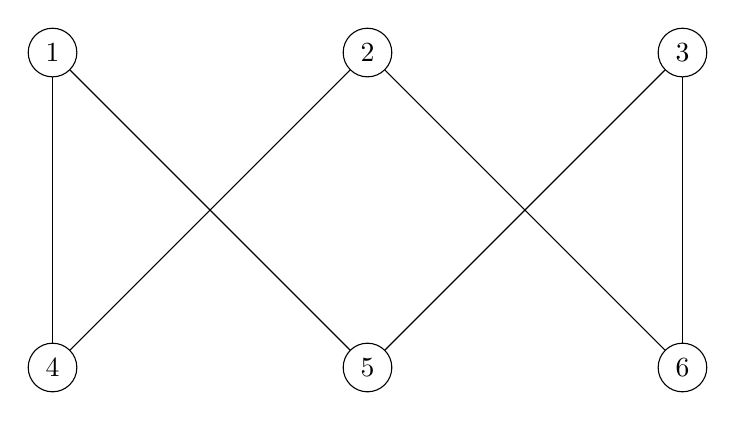
\begin{tikzpicture}[node distance={40mm}, main/.style = {draw, circle}] 
\node[main] (1) {$1$}; 
\node[main] (2) [right of=1] {$2$}; 
\node[main] (3) [right of=2] {$3$}; 
\node[main] (4) [below of=1] {$4$}; 
\node[main] (5) [below of=2] {$5$}; 
\node[main] (6) [below of=3] {$6$}; 

\draw (1) -- (4); 
\draw (1) -- (5); 
\draw (2) -- (4); 
\draw (2) -- (6); 
\draw (3) -- (5); 
\draw (3) -- (6); 
\end{tikzpicture} 
\end{center}
У даному випадку ми можемо розділити множину вершин на дві:
\begin{center}
$V = U \cup P, P = \{1,2,3\}$ та $U = \{4,5,6\}$.
\end{center}
Немає жодного ребра яке пов'язує вершини множин $P$ із вершинами множини $P$, аналогічно для множини $U$.
\end{example}

\begin{theorem}
В дводольному графі для будь-якого натурального $k$ будь-які вершини однієї долі, де $k$ не перевищує числа вершин доль, пов'язані принаймні з $k$ різними вершинами іншої долі тоді і лише тоді, коли граф розбивається на пари першою часткою.
\end{theorem}

\section{Постановка задачі}

\begin{theorem}
Довести {\bf Теорему 1} у тому вигляді, у якому вона описана, зважаючи лише на те що об'єкт $M$ у твердженні теореми тепер може мати мультимножинну природу.
\end{theorem}

\begin{proof}
Використаємо підхід, який базується на {\bf Теоремі 2}. У даному доведенні буде описуватись один з можливих підходів рішення та доведення {\bf даної теореми} через навантаження ребер двочасткового графу певними коефіцієнтами.
У моїй бакалаврській роботі було розглянуто такі випадки: 
\begin{center}
$A = \{z^m,x^m\}, B = \{w_0^{2}, w_1,...,w_n\}$
\end{center}

Як вже було доведено раніше у {\bf Теоремі 1} для звичайного типу множин завжди існує паросполучення при додаванні до сімейства невкладених множин розміру $n$ одного елемента для того, щоб утворити сімейство невкладених множин якому належать множини розміру $n+1$. Для звичайного випадка теореми це і доводить, що максимально можливий розмір такого сімейства ${C_n}^{[n/2]}$. Для випадка коли множина має мультимножинну природу використати {\bf Теорему 1} у тому вигляді як описано вище неможливо.

\begin{example}

Розглянемо множину $ A = \{2,3,4\} $, збудуємо наповнення одноелементного сімейства невключних одна в одну множин, які добудуємо до двоелементного сімейства:

\begin{center}
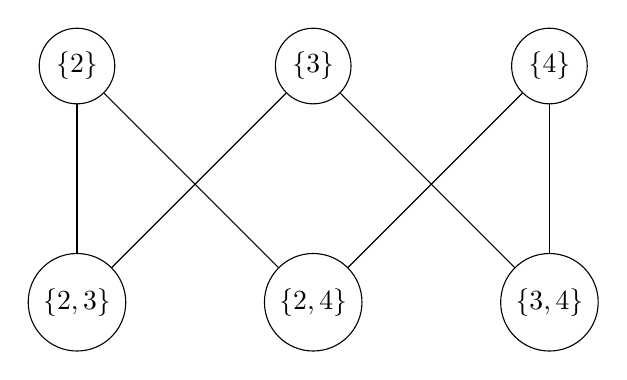
\begin{tikzpicture}[node distance={30mm}, main/.style = {draw, circle}] 
\node[main] (1) {$\{2\}$}; 
\node[main] (2) [right of=1] {$\{3\}$}; 
\node[main] (3) [right of=2] {$\{4\}$}; 
\node[main] (4) [below of=1] {$\{2,3\}$}; 
\node[main] (5) [below of=2] {$\{2,4\}$}; 
\node[main] (6) [below of=3] {$\{3,4\}$}; 

\draw (1) -- (4); 
\draw (1) -- (5); 
\draw (2) -- (4); 
\draw (2) -- (6); 
\draw (3) -- (5); 
\draw (3) -- (6); 
\end{tikzpicture} 
\end{center}
\end{example}

Ідея полягає в тому, щоб перенести підхід паросполучення використовуючи вагові коефіцієнти.
Як можна бачити з малюнка:
\begin{center}
$ \underline{deg} = t $
\\
$ \overline{deg} = n - t $
\end{center}
Але це можливо лише для випадку коли відповідні ребра навантажені вагами. Нижче буде розглянуто декілька прикладів для розуміння повної картини.
\end{proof}


\begin{example}

Розглянемо множину $ A = \{2^3,3^2\} $, збудуємо наповнення двоелементного сімейства невключних одна в одну множин, які добудуємо до триелементного сімейства:

\begin{center}
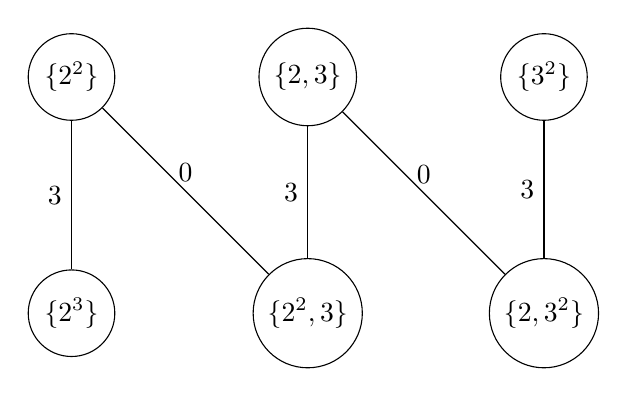
\begin{tikzpicture}[node distance={30mm}, main/.style = {draw, circle}] 
\node[main] (1) {$\{2^2\}$}; 
\node[main] (2) [right of=1] {$\{2,3\}$}; 
\node[main] (3) [right of=2] {$\{3^2\}$}; 
\node[main] (4) [below of=1] {$\{2^3\}$}; 
\node[main] (5) [below of=2] {$\{2^2,3\}$}; 
\node[main] (6) [below of=3] {$\{2,3^2\}$}; 

\draw (1) -- node[left] {3} (4); 
\draw (1) -- node[above] {0} (5); 
\draw (2) -- node[left] {3} (5); 
\draw (2) -- node[above] {0} (6); 
\draw (3) -- node[left] {3} (6); 
\end{tikzpicture} 
\end{center}

\end{example}

\newpage

\begin{example}

Розглянемо множину $ A = \{2^3,3^3\} $, також збудуємо наповнення двоелементного сімейства невключних одна в одну множин, які добудуємо до триелементного сімейства:

\begin{center}
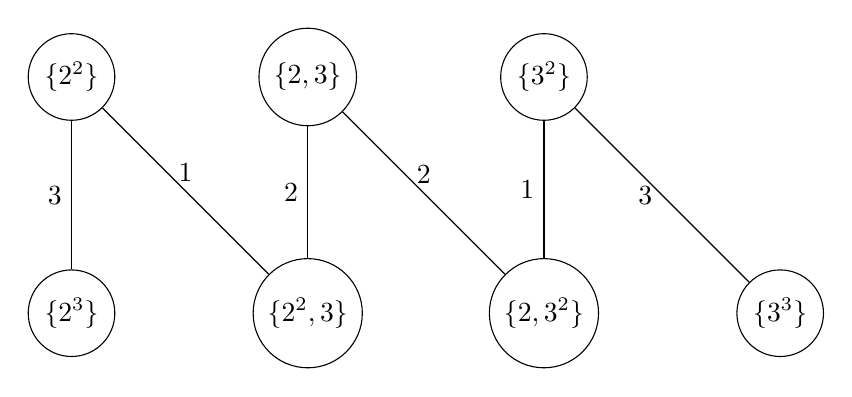
\begin{tikzpicture}[node distance={30mm}, main/.style = {draw, circle}] 
\node[main] (1) {$\{2^2\}$}; 
\node[main] (2) [right of=1] {$\{2,3\}$}; 
\node[main] (3) [right of=2] {$\{3^2\}$}; 
\node[main] (4) [below of=1] {$\{2^3\}$}; 
\node[main] (5) [below of=2] {$\{2^2,3\}$};
\node[main] (6) [below of=3] {$\{2,3^2\}$}; 
\node[main] (7) [right of=6] {$\{3^3\}$}; 

\draw (1) -- node[left]  {3} (4); 
\draw (1) -- node[above] {1} (5); 
\draw (2) -- node[left]  {2} (5); 
\draw (2) -- node[above] {2} (6); 
\draw (3) -- node[left]  {1} (6); 
\draw (3) -- node[left]  {3} (7); 
\end{tikzpicture} 
\end{center}
\end{example}

Тобто обрахунок ведеться за допомогою формул:
\begin{center}
$ \underline{deg} = t $
\\
$ \overline{deg} = n - t $
\end{center}
$n$ - мультипотужність множини на основі якої будується сімейство невкладених одна в одну множин
\\
$t$ - мультипотужність множини яка належить сімейству невкладених одна в одну множин (для $\underline{deg}
$, $t$ - це потужність множини яка належить нижній долі, для  $\overline{deg}$, $t$ - це потужність множини яка належить верхній долі)

Тобто для {\bf Прикладу 4}:
\begin{center}
$ \underline{deg} = 3 $ - оскільки $ |\{2^3\}| = |\{2^2,3\}| = |\{2,3^2\}| $
\\
$ \overline{deg} = |A| - 2 = 3 $ - оскільки $ |A| = 5, |\{2^2\}| = |\{2,3\}| = |\{3^2\}| = 2 $
\end{center}
Далі складається система лінійних рівнянь:

\begin{center}
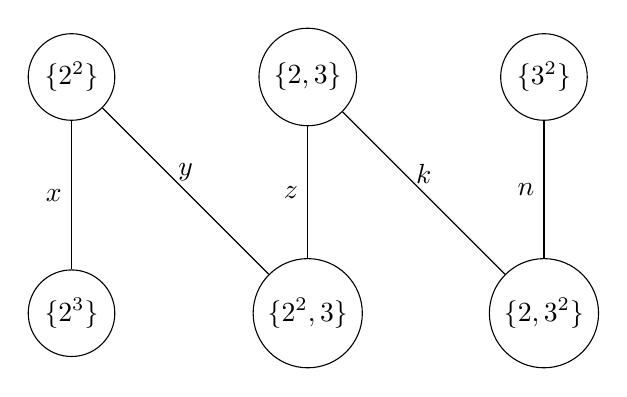
\begin{tikzpicture}[node distance={30mm}, main/.style = {draw, circle}] 
\node[main] (1) {$\{2^2\}$}; 
\node[main] (2) [right of=1] {$\{2,3\}$}; 
\node[main] (3) [right of=2] {$\{3^2\}$}; 
\node[main] (4) [below of=1] {$\{2^3\}$}; 
\node[main] (5) [below of=2] {$\{2^2,3\}$}; 
\node[main] (6) [below of=3] {$\{2,3^2\}$}; 

\draw (1) -- node[left] {$x$} (4); 
\draw (1) -- node[above] {$y$} (5); 
\draw (2) -- node[left] {$z$} (5); 
\draw (2) -- node[above] {$k$} (6); 
\draw (3) -- node[left] {$n$} (6); 
\end{tikzpicture} 
\end{center}
\begin{center}
$\left \{
\begin{tabular}{ccc}
x = 3 \\
x + y = 3 \\ 
y + z = 3 \\
z + k = 3 \\ 
k + n = 3 
  \end{tabular}
    \Rightarrow 
$
$
\left \{
  \begin{tabular}{ccc}
x = 3 \\
y = 0 \\ 
z = 3 \\
k = 0 \\ 
n = 3 
  \end{tabular}
$
\end{center}

Для {\bf Прикладу 5}:
\begin{center}
$ \underline{deg} = 3 $ - оскільки $ |\{2^3\}| = |\{2^2,3\}| = |\{3^3\}| $
\\
$ \overline{deg} = |A| - 2 = 4 $ - оскільки $ |A| = 6, |\{2^2\}| = |\{2,3\}| = |\{3^2\}| = 2 $
\end{center}
Далі складається система лінійних рівнянь:

\begin{center}
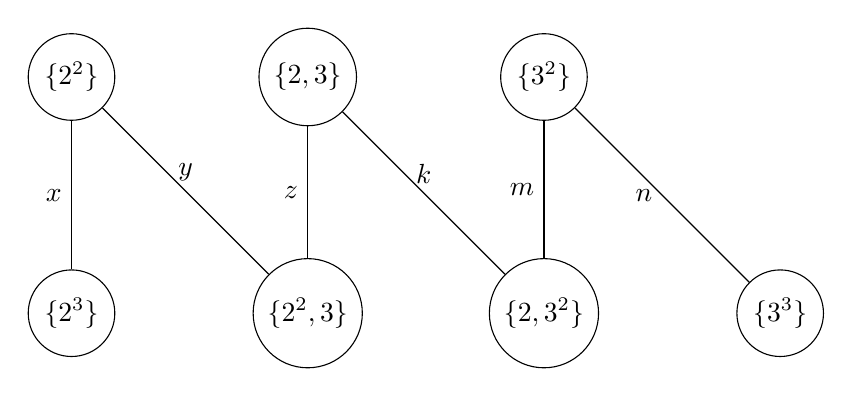
\begin{tikzpicture}[node distance={30mm}, main/.style = {draw, circle}] 
\node[main] (1) {$\{2^2\}$}; 
\node[main] (2) [right of=1] {$\{2,3\}$}; 
\node[main] (3) [right of=2] {$\{3^2\}$}; 
\node[main] (4) [below of=1] {$\{2^3\}$}; 
\node[main] (5) [below of=2] {$\{2^2,3\}$};
\node[main] (6) [below of=3] {$\{2,3^2\}$}; 
\node[main] (7) [right of=6] {$\{3^3\}$}; 

\draw (1) -- node[left]  {$x$} (4); 
\draw (1) -- node[above] {$y$} (5); 
\draw (2) -- node[left]  {$z$} (5); 
\draw (2) -- node[above] {$k$} (6); 
\draw (3) -- node[left]  {$m$} (6); 
\draw (3) -- node[left]  {$n$} (7); 
\end{tikzpicture} 
\end{center}

\begin{center}
$\left \{
\begin{tabular}{ccc}
x = 3 \\
x + y = 4 \\ 
y + z = 3 \\
z + k = 4 \\ 
k + m = 3 \\ 
n = 3 
  \end{tabular}
    \Rightarrow 
$
$
\left \{
  \begin{tabular}{ccc}
x = 3 \\
y = 1 \\ 
z = 2 \\
k = 2 \\ 
m = 1 \\
n = 3
 
  \end{tabular}
$
\end{center}

Таким способом у бакалаврській роботі було доведено випадки $A = \{z^m,x^m\}, B = \{w_0^{2}, w_1,...,w_n\}$. У наступному розділі буде розглянуто декілька інших часткових випадків, для яких буде доведено {\bf Теорему 1}, та будуть записані явні формули обрахунку вагів для графу. За допомогою цих формул можна переконатись, що паросполучення існує і побудувати його явно. Таким чином доводиться для множин мультимножинної природи справедливість {\bf Теореми 1}. Прикладе застосування математичних об'єктів, які задовольняють умови теореми буде описано у роздулах пізніше.

\newpage

\chapter{Часткові випадки теореми}
\section{Частковий випадок $A = \{a^m, b, c\}$}

Ми почнемо розглядати новий випадок мультимножини виду $A = \{a^m, b, c\}$, яка задовольняє умови {\bf Теореми 1}. На елемент $a^m$ накладаються деякі обмеження, а саме: $m \geq 3 $, оскільки при $ m = 1 $ висхідна множина втрачає мультимножинні властивості, щодо випадку коли  $ m = 2 $, то цей випадок вже був розглянутий у бакалаврській роботі, та включається у випадок $B = \{w_0^{2}, w_1,...,w_n\}$. Почнемо з частинних випадків коли  $ m $ набуває конкретних значень, щоб побачити закономірності у зажуванні дводольного графу та формули за допомогою яких будуть обраховуватись ваги.

\begin{example}

Розглянемо множину $ A = \{a^3, b, c\} $, збудуємо наповнення двоелементного сімейства невключних одна в одну множин, які добудуємо до триелементного сімейства:

\begin{center}
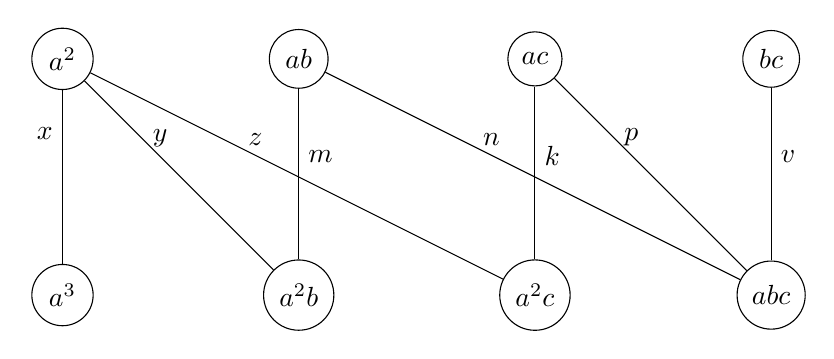
\begin{tikzpicture}[node distance={30mm}, main/.style = {draw, circle}] 
\node[main] (1) {$a^2$}; 
\node[main] (2) [right of=1] {$ab$}; 
\node[main] (3) [right of=2] {$ac$}; 
\node[main] (4) [right of=3] {$bc$}; 
\node[main] (5) [below of=1] {$a^3$}; 
\node[main] (6) [below of=2] {$a^2b$}; 
\node[main] (7) [below of=3] {$a^2c$}; 
\node[main] (8) [below of=4] {$abc$}; 

\draw (1) -- node[pos=0.25, left] {$x$} (5); 
\draw (1) -- node[pos=0.4, above] {$y$} (6); 
\draw (1) -- node[pos=0.4, above] {$z$} (7); 

\draw (2) -- node[pos=0.4, right] {$m$}(6); 
\draw (2) -- node[pos=0.4, above] {$n$}(8); 

\draw (3) -- node[pos=0.4, right] {$k$}(7); 
\draw (3) -- node[pos=0.4, above] {$p$}(8); 
\draw (4) -- node[pos=0.4, right] {$v$}(8); 
\end{tikzpicture} 
\end{center}
\end{example}

Так само, як і у випадках раніше підрахуємо значення вагів за формулою:
\begin{center}
$ \underline{deg} = 3 $ - оскільки $ |\{a^3\}| = |\{a^2,b\}| = |\{a^2,c\}| = |\{a,b,c\}| $
\\
$ \overline{deg} = |A| - 2 = 3 $ - оскільки $ |A| = 5, |\{a^2\}| = |\{a,b\}| = |\{b,c\}| =  |\{a,c\}| = 2 $
\end{center}

\begin{center}
$\left \{
\begin{tabular}{ccc}
x = 3 \\
x + y + z = 3 \\ 
m + y = 3 \\
m + n = 3 \\
z + k = 3 \\
k + p = 3 \\
n + p + v = 3 \\ 
v = 3 
  \end{tabular}
    \Rightarrow 
$
$
\left \{
  \begin{tabular}{ccc}
x = 3 \\
y = 0 \\ 
z = 0 \\
m = 3 \\ 
n = 0 \\
k = 3 \\
p = 0 \\
v = 3
 
  \end{tabular}
$
\end{center}

Для випадку коли  вага ребра дорівнює $ 0 $, ми виключаємо таке ребро із графу, тобто ми отримали повне паросполучення:
\begin{center}
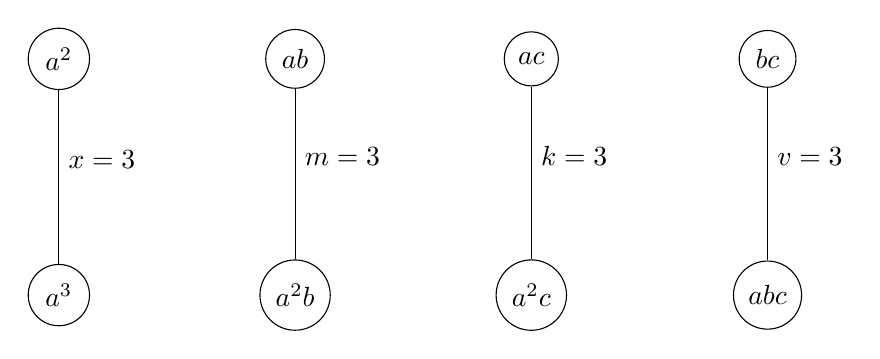
\begin{tikzpicture}[node distance={30mm}, main/.style = {draw, circle}] 
\node[main] (1) {$a^2$}; 
\node[main] (2) [right of=1] {$ab$}; 
\node[main] (3) [right of=2] {$ac$}; 
\node[main] (4) [right of=3] {$bc$}; 
\node[main] (5) [below of=1] {$a^3$}; 
\node[main] (6) [below of=2] {$a^2b$}; 
\node[main] (7) [below of=3] {$a^2c$}; 
\node[main] (8) [below of=4] {$abc$}; 

\draw (1) -- node[pos=0.4,right] {$x = 3$}(5); 
\draw (2) -- node[pos=0.4, right] {$m = 3$}(6); 
\draw (3) -- node[pos=0.4, right] {$k = 3$}(7); 
\draw (4) -- node[pos=0.4, right] {$v = 3$}(8); 
\end{tikzpicture} 
\end{center}


\begin{example}

Розглянемо множину $ A = \{a^4, b, c\} $, так само збудуємо наповнення двоелементного сімейства невключних одна в одну множин, які добудуємо до триелементного сімейства:

\begin{center}
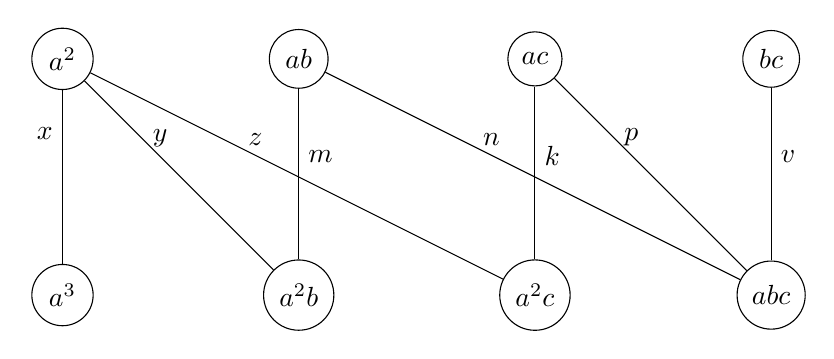
\begin{tikzpicture}[node distance={30mm}, main/.style = {draw, circle}] 
\node[main] (1) {$a^2$}; 
\node[main] (2) [right of=1] {$ab$}; 
\node[main] (3) [right of=2] {$ac$}; 
\node[main] (4) [right of=3] {$bc$}; 
\node[main] (5) [below of=1] {$a^3$}; 
\node[main] (6) [below of=2] {$a^2b$}; 
\node[main] (7) [below of=3] {$a^2c$}; 
\node[main] (8) [below of=4] {$abc$}; 

\draw (1) -- node[pos=0.25, left] {$x$} (5); 
\draw (1) -- node[pos=0.4, above] {$y$} (6); 
\draw (1) -- node[pos=0.4, above] {$z$} (7); 

\draw (2) -- node[pos=0.4, right] {$m$}(6); 
\draw (2) -- node[pos=0.4, above] {$n$}(8); 

\draw (3) -- node[pos=0.4, right] {$k$}(7); 
\draw (3) -- node[pos=0.4, above] {$p$}(8); 
\draw (4) -- node[pos=0.4, right] {$v$}(8); 
\end{tikzpicture} 
\end{center}
\end{example}

Так само як для попереднього випадку:
\begin{center}
$ \underline{deg} = 3 $ - оскільки $ |\{a^3\}| = |\{a^2,b\}| = |\{a^2,c\}| = |\{a,b,c\}| $
\\
$ \overline{deg} = |A| - 2 = 3 $ - оскільки $ |A| = 5, |\{a^2\}| = |\{a,b\}| = |\{b,c\}| =  |\{a,c\}| = 2 $
\end{center}

\begin{center}
$\left \{
\begin{tabular}{ccc}
x = 3 \\
x + y + z = 3 \\ 
m + y = 3 \\
m + n = 3 \\
z + k = 3 \\
k + p = 3 \\
n + p + v = 3 \\ 
v = 3 
  \end{tabular}
    \Rightarrow 
$
$
\left \{
  \begin{tabular}{ccc}
x = 3 \\
y = 0 \\ 
z = 0 \\
m = 3 \\ 
n = 0 \\
k = 3 \\
p = 0 \\
v = 3
 
  \end{tabular}
$
\end{center}

Для випадку коли  вага ребра дорівнює $ 0 $, ми виключаємо таке ребро із графу, тобто ми отримали повне паросполучення:
\begin{center}
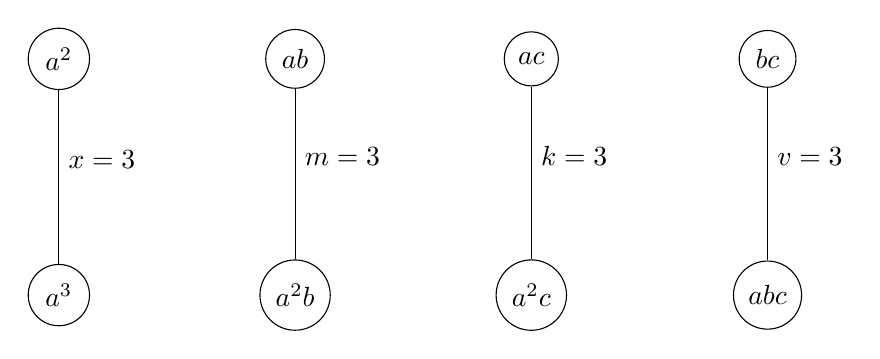
\begin{tikzpicture}[node distance={30mm}, main/.style = {draw, circle}] 
\node[main] (1) {$a^2$}; 
\node[main] (2) [right of=1] {$ab$}; 
\node[main] (3) [right of=2] {$ac$}; 
\node[main] (4) [right of=3] {$bc$}; 
\node[main] (5) [below of=1] {$a^3$}; 
\node[main] (6) [below of=2] {$a^2b$}; 
\node[main] (7) [below of=3] {$a^2c$}; 
\node[main] (8) [below of=4] {$abc$}; 

\draw (1) -- node[pos=0.4,right] {$x = 3$}(5); 
\draw (2) -- node[pos=0.4, right] {$m = 3$}(6); 
\draw (3) -- node[pos=0.4, right] {$k = 3$}(7); 
\draw (4) -- node[pos=0.4, right] {$v = 3$}(8); 
\end{tikzpicture} 
\end{center}

Ми отримали точно такий же граф, як і у попередньому випадку, навіть з такими же вагами. Давайте спробуємо узагальнити підхід для випадку коли $ A = \{a^m, b, c\} $. Я буду спиратись на твердження, яке було доведене у моїй бакалаврській роботі:

\begin{center}
$ C_n^{k} \leq C_n^{k+1} $, для випадку коли $ k < [n/2]$, де $n$ - це кількість елементів висхідної множини, $k$ - потужність підмножини.
\end{center}

Отже, за припущенням найбільше сімейство мультипідможин, які невключаються одна в одну, тобто максимальна потужність такого сімейства набувається коли потужність кожної окремої множини дорівнює $ [n/2] $. $|A| = m + 2$, тоді побудуємо перехід від $ [(m+2)/2 - 1]$ елементних підмножин до $ [(m+2)/2]$:

Розглянемо множину $ A = \{a^m, b, c\} $, так само збудуємо наповнення двоелементного сімейства невключних одна в одну множин, які добудуємо до триелементного сімейства:

\begin{center}
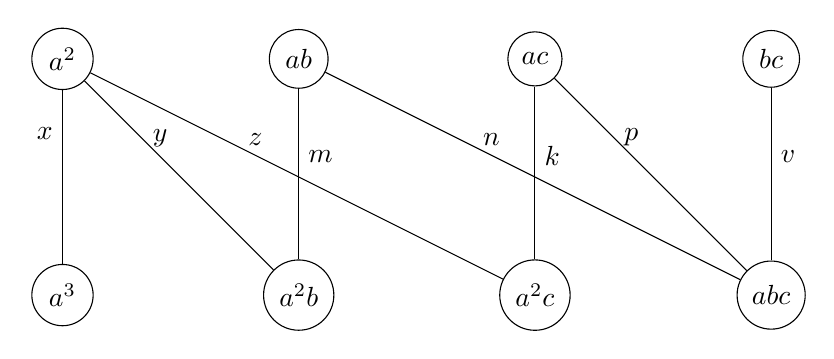
\begin{tikzpicture}[node distance={30mm}, main/.style = {draw, circle}] 
\node[main] (1) {$a^2$}; 
\node[main] (2) [right of=1] {$ab$}; 
\node[main] (3) [right of=2] {$ac$}; 
\node[main] (4) [right of=3] {$bc$}; 
\node[main] (5) [below of=1] {$a^3$}; 
\node[main] (6) [below of=2] {$a^2b$}; 
\node[main] (7) [below of=3] {$a^2c$}; 
\node[main] (8) [below of=4] {$abc$}; 

\draw (1) -- node[pos=0.25, left] {$x$} (5); 
\draw (1) -- node[pos=0.4, above] {$y$} (6); 
\draw (1) -- node[pos=0.4, above] {$z$} (7); 

\draw (2) -- node[pos=0.4, right] {$m$}(6); 
\draw (2) -- node[pos=0.4, above] {$n$}(8); 

\draw (3) -- node[pos=0.4, right] {$k$}(7); 
\draw (3) -- node[pos=0.4, above] {$p$}(8); 
\draw (4) -- node[pos=0.4, right] {$v$}(8); 
\end{tikzpicture} 
\end{center}
\end{example}

Так само як для попереднього випадку:
\begin{center}
$ \underline{deg} = 3 $ - оскільки $ |\{a^3\}| = |\{a^2,b\}| = |\{a^2,c\}| = |\{a,b,c\}| $
\\
$ \overline{deg} = |A| - 2 = 3 $ - оскільки $ |A| = 5, |\{a^2\}| = |\{a,b\}| = |\{b,c\}| =  |\{a,c\}| = 2 $
\end{center}

\begin{center}
$\left \{
\begin{tabular}{ccc}
x = 3 \\
x + y + z = 3 \\ 
m + y = 3 \\
m + n = 3 \\
z + k = 3 \\
k + p = 3 \\
n + p + v = 3 \\ 
v = 3 
  \end{tabular}
    \Rightarrow 
$
$
\left \{
  \begin{tabular}{ccc}
x = 3 \\
y = 0 \\ 
z = 0 \\
m = 3 \\ 
n = 0 \\
k = 3 \\
p = 0 \\
v = 3
 
  \end{tabular}
$
\end{center}

Для випадку коли  вага ребра дорівнює $ 0 $, ми виключаємо таке ребро із графу, тобто ми отримали повне паросполучення:
\begin{center}
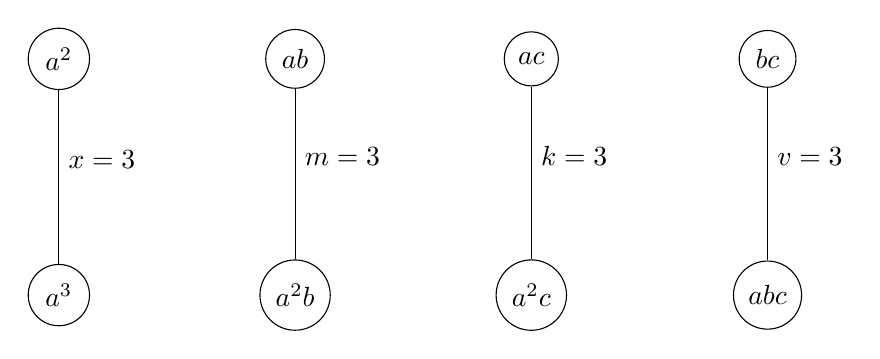
\begin{tikzpicture}[node distance={30mm}, main/.style = {draw, circle}] 
\node[main] (1) {$a^2$}; 
\node[main] (2) [right of=1] {$ab$}; 
\node[main] (3) [right of=2] {$ac$}; 
\node[main] (4) [right of=3] {$bc$}; 
\node[main] (5) [below of=1] {$a^3$}; 
\node[main] (6) [below of=2] {$a^2b$}; 
\node[main] (7) [below of=3] {$a^2c$}; 
\node[main] (8) [below of=4] {$abc$}; 

\draw (1) -- node[pos=0.4,right] {$x = 3$}(5); 
\draw (2) -- node[pos=0.4, right] {$m = 3$}(6); 
\draw (3) -- node[pos=0.4, right] {$k = 3$}(7); 
\draw (4) -- node[pos=0.4, right] {$v = 3$}(8); 
\end{tikzpicture} 
\end{center}

\section{Частковий випадок $A = \{a^m, b^2, c\}$}


\newpage


\subsection{Попередні роботи} 
\subsection{Визначення}
\section{Практичне застосування}
